\documentclass[12pt,]{article}
\usepackage[utf8]{inputenc}
\usepackage[T1]{fontenc}
\usepackage{mathptmx}
\usepackage{geometry}
\usepackage{mathtools}
\usepackage[english]{babel}
\usepackage{graphicx}
\usepackage{stackengine}
\usepackage[os=win]{menukeys}
\usepackage{hyperref}
\usepackage{minted}
\usepackage{xcolor}
\usepackage{tikz}
\usepackage[yyyymmdd,hhmmss]{datetime}
\usepackage{etoolbox}
\usepackage{enumitem}

\patchcmd{\thebibliography}{\section*{\refname}}{}{}{}

\newcommand{\ShowOsVersion}{
	\immediate\write18{\unexpanded{foo=`uname -sro` && echo "${foo}" > tmp.tex}}
	\input{tmp}\immediate\write18{rm tmp.tex}
}

\newcommand{\ShowTexVersion}{
	\immediate\write18{\unexpanded{foo=`pdflatex -version | head -n1 | cut -d' ' -f1,2` && echo "${foo}" > tmp.tex}}
	\input{tmp}\immediate\write18{rm tmp.tex}
}

\addto\captionsenglish{\renewcommand{\contentsname}{Daftar Isi}}

\hypersetup{
	colorlinks=true, %set true if you want colored links
	linktoc=all,     %set to all if you want both sections and subsections linked
	linkcolor=blue,  %choose some color if you want links to stand out
	urlcolor=blue,	 %url color
}

\geometry{
	legalpaper,
	left=15mm,
	right=10mm,
	top=10mm,
	bottom=15mm,
}

\title{\Large \bf
	Patent Claim Draft\\
}

\author{Achmadi ST MT}

\date{}

\hypersetup{citecolor=black}

\definecolor{LightGray}{gray}{0.95}

%\pagecolor[rgb]{0.1,0.1,0.1}
%\color[rgb]{1,1,1}

\begin{document}
	\maketitle
	\thispagestyle{empty}
	
	\newpage
	\section{Daftar Klaim}
	
	\subsection{Fitur Utama}
	
	Berikut fitur utama dan penempatannya:
	\begin{enumerate}
		\item Power Switch, untuk mematikan/menghidupkan unit.
		\item Jack Audio 3.5mm, untuk output ke headphone.
		\item Tombol-tombol, untuk interaksi user.
		\item Lampu-lampu LED, untuk interaksi user.
		\item Lampu indikator jawaban salah-benar.
		\item Port USB untuk Charging
		\item Tombol Reset, untuk memulai ulang unit
		\item Lampu LED Indikator Mode
		\item Slot Memory MicroSD
		\item Port USB untuk koneksi data dengan PC/Android
	\end{enumerate}

	\begin{figure}[!ht]
		\centering
		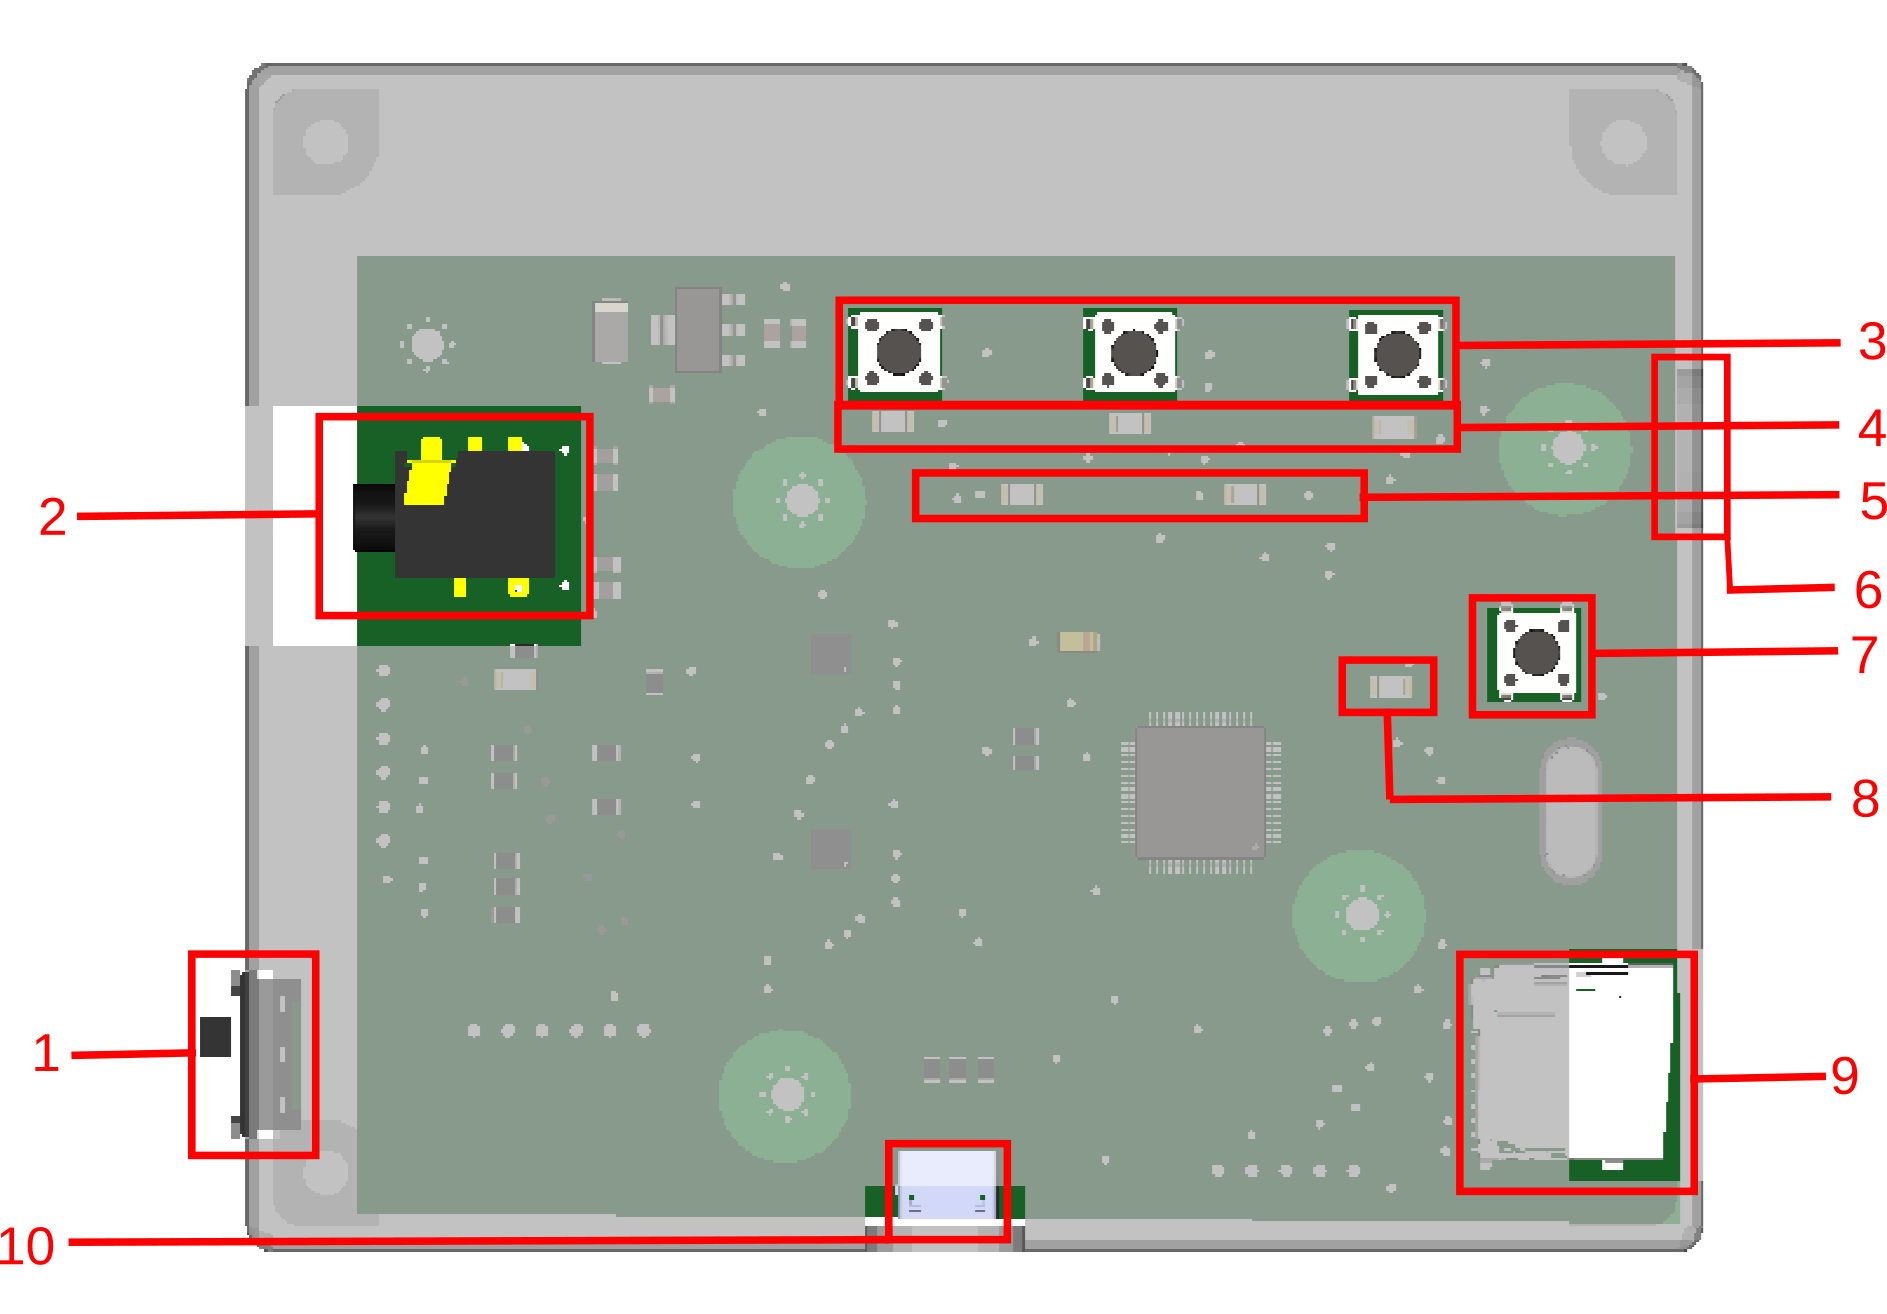
\includegraphics[width=400pt]{images/fig_1_part}
		\caption{Layout penempatan fitur-fitur untuk interaksi dengan pengguna}
	\end{figure}

	\textbf{Poin Klaim:} Pola penempatan (layout) fitur-fitur pada box sedemikian ditunjukkan oleh Figure 1.
	
	\newpage
	\subsection{Start Sequence}
	
	Berikut urutan langkah mudah untuk memulai proses Audiometri pada unit
	\begin{enumerate}
		\item Pastikan bahwa unit Audimetri pada status siap.
		\begin{enumerate}
			\renewcommand{\theenumi}{\Alph{enumi}}
			
			\item Nyalakan unit pada switch power
			\item Headphone telah tersambung
			\item MicroSD telah terpasang
		\end{enumerate}
	
		\item LED Mode akan berkedip satu kali setiap satu detik
		\item Tekan satu kali tombol nomor 3 
		\item LED Indikator nomor 4 akan menyala
		\item Tekan satu kali tombol nomor 5
		\item LED nomer 4 akan mati dan LED nomor 6 akan menyala
		\item Tekan satu kali tombol nomor 7
		\item Semua LED akan mati kecuali LED nomor 2 atau 8 akan berkedip cepat.
	\end{enumerate}

	Proses Audiometri telah dimulai.

	\begin{figure}[!ht]
		\centering
		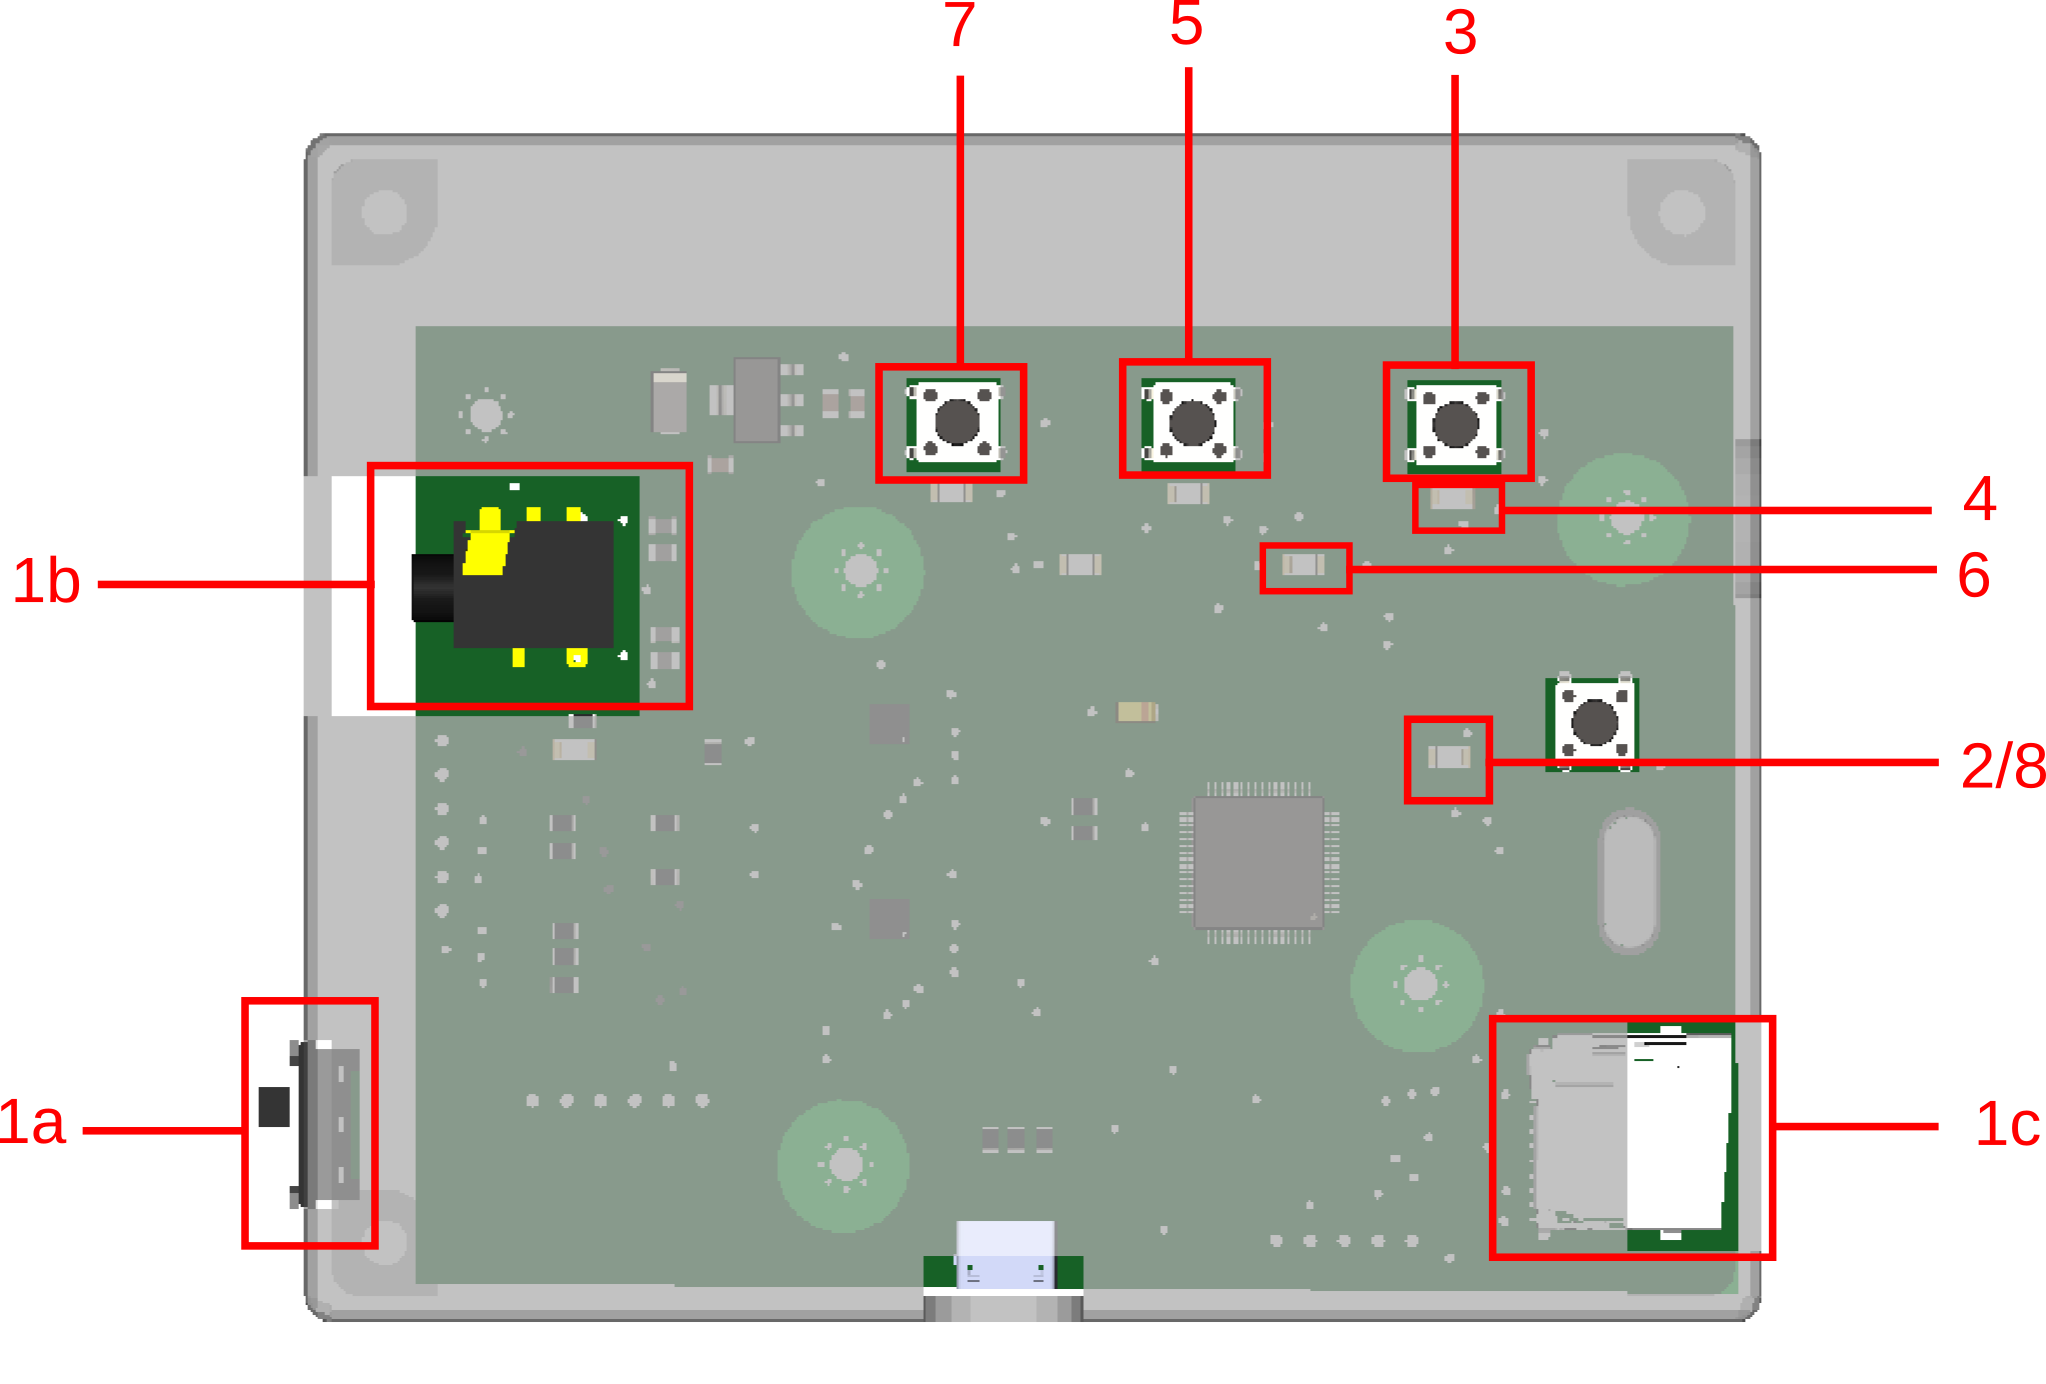
\includegraphics[width=400pt]{images/fig_2_startup}
		\caption{Urutan langkah memulai proses Audiometri}
	\end{figure}

	\textbf{Poin Klaim:} Urutan langkah interaksi pengguna untuk memulai proses Audimetri sebagaimana dijelaskan
	pada penjelasan di atas dan pada Figure 2
	
	\newpage
	\subsection{Interaksi Audiometri}
	
	Berikut adalah urutan langkah interaksi pengguna saat proses Audiometri.
	\begin{enumerate}
		\item Pastikan poin berikut telah siap. Jika belum maka reset kembali unit
		dan ulangi kembali langkah startup.
		\begin{enumerate}
			\renewcommand{\theenumi}{\Alph{enumi}}
			
			\item LED Indikator pada posisi 1a berkedip cepat.
			\item Headphone telah terpasang.
		\end{enumerate}
	
		\item \textbf{Perhatikan} output dari unit.
		\begin{enumerate}
			\renewcommand{\theenumi}{\Alph{enumi}}
			
			\item LED pada baris 2a akan berkedip sekali bergantian
			\item Nada murni pada output 2a akan terdengar,
			bersamaan salah satu LED baris 2a.
		\end{enumerate}
	
		\item Tekan satu tombol dimana LED baris 2a menyala bersamaan dengan terdengar nada murni.
		
		\item LED pada baris 4 akan menyala sebagai respon jawaban.
		Hijau jika benar atau Merah jika salah.
		
		\item Lanjutkan hingga LED Mode pada nomor 5 kembali berkedip satu setiap satu detik,
		yang menandakan sesi uji Audiometri selesai.
	\end{enumerate}
	
	\begin{figure}[!ht]
		\centering
		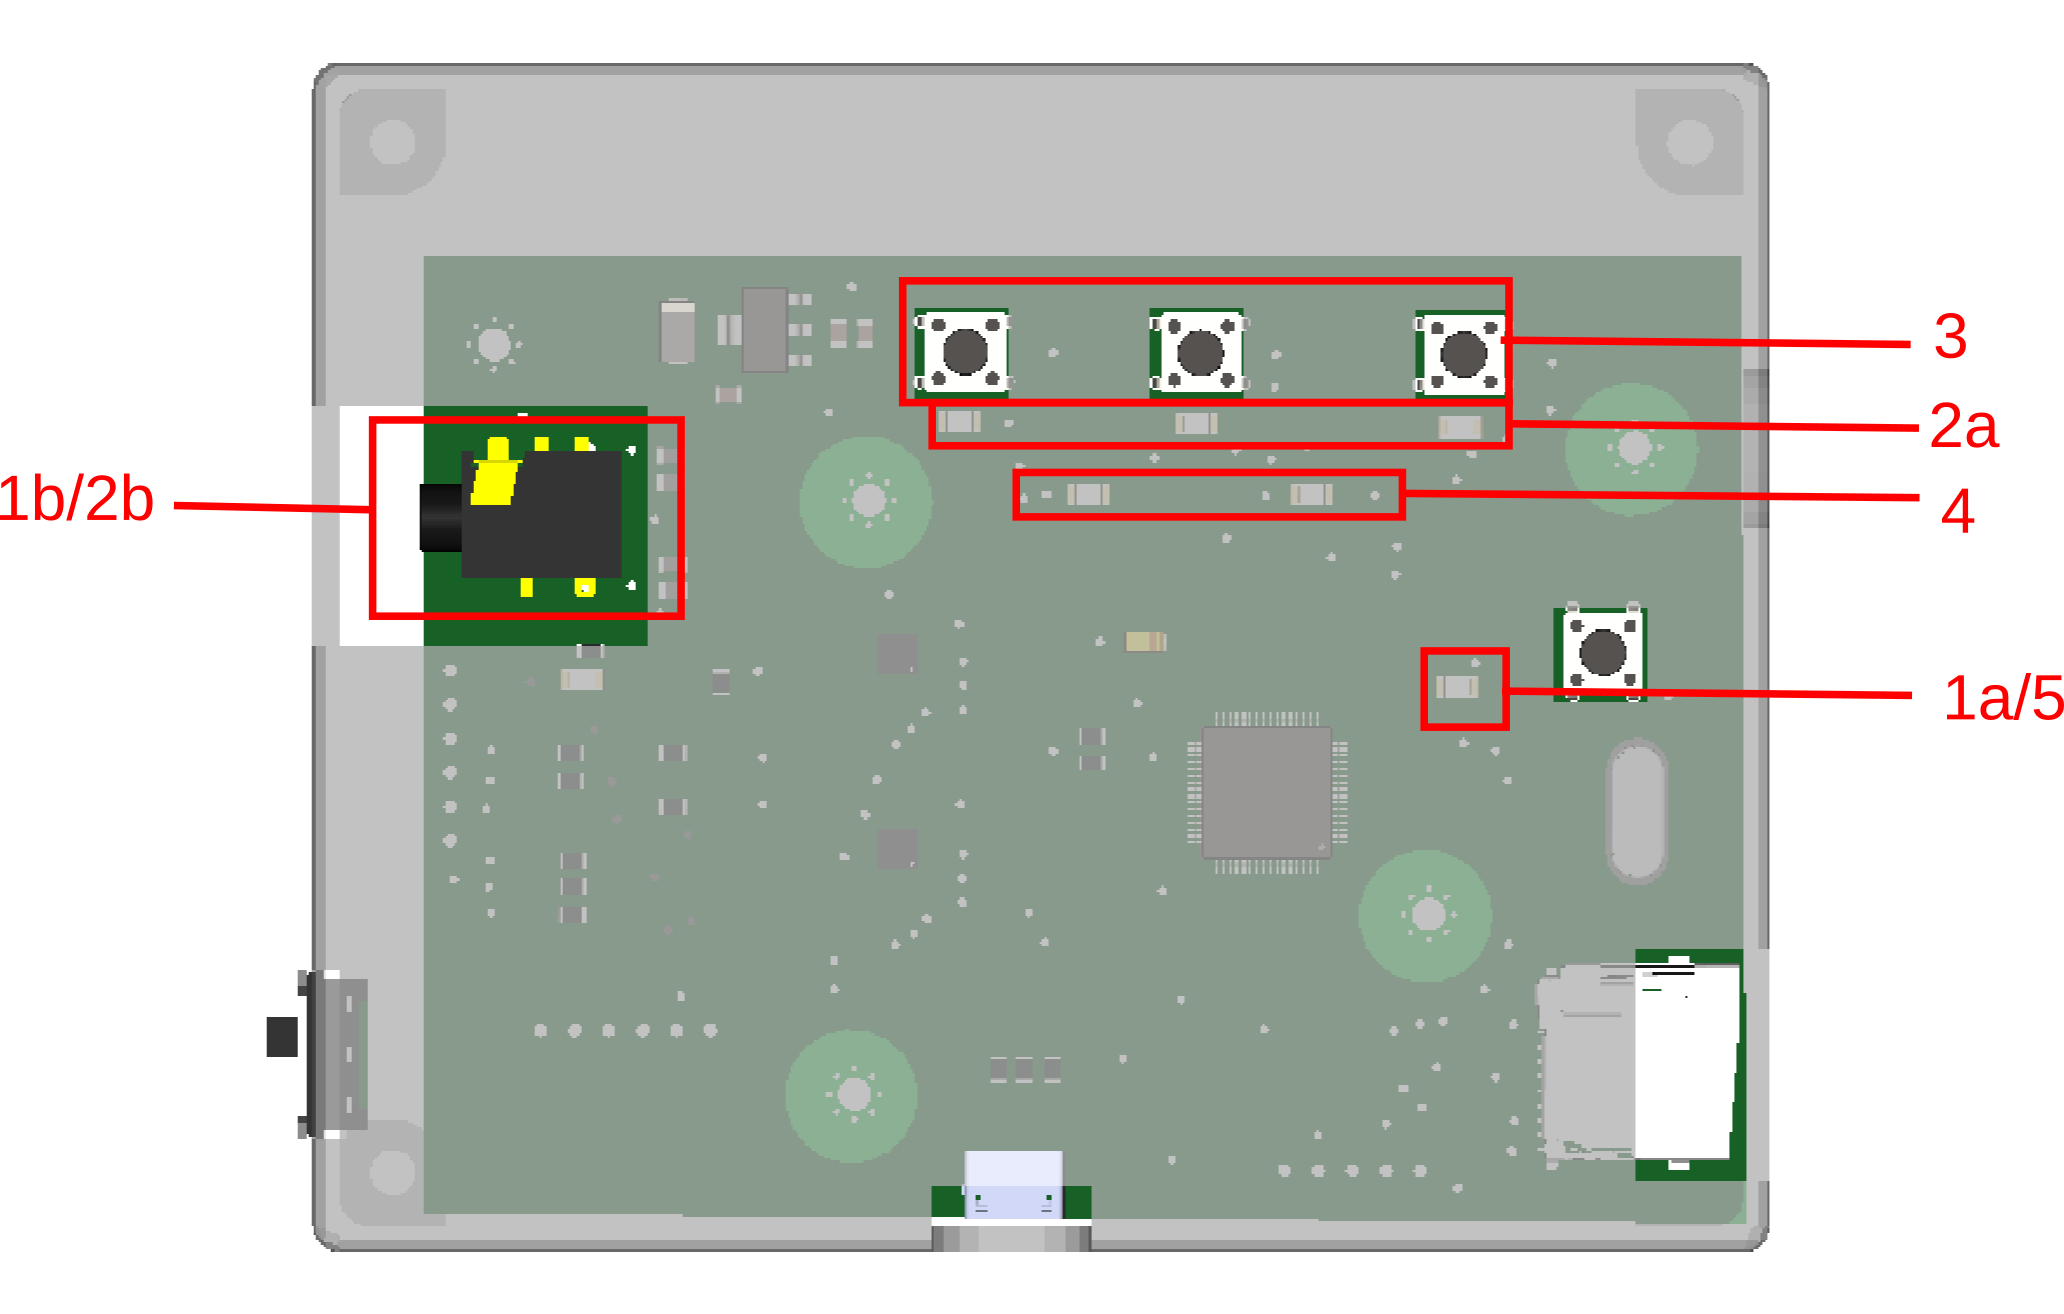
\includegraphics[width=400pt]{images/fig_3_metri}
		\caption{Interaksi Proses Audiometri}
	\end{figure}

	\textbf{Poin Klaim:} Urutan langkah interaksi pengguna untuk selama proses Audimetri sebagaimana dijelaskan
	pada penjelasan di atas dan pada Figure 3.
	
	\newpage
	\subsection{Merek dan Logo}
	
	Belum terdefinisi dan bukan poin klaim Paten melainkan Merek Dagang.
	
\end{document}